\documentclass[aspectratio=169, 10pt]{beamer}
\usepackage[utf8]{inputenc}
\usepackage[vietnamese]{babel}
\usepackage{graphicx}
\usepackage{amsmath}
\usepackage{amssymb}
\usepackage{booktabs}
\usepackage{hyperref}
\usepackage{tabularx}
\usepackage{colortbl}
\usepackage{tcolorbox}
\usepackage{algorithmic}

\usetheme{Madrid}
\usecolortheme{default}

\title[Training-Free Style-Personalization]{A Training-Free Style-Personalization \\ via SVD-Based Feature Decomposition}
\subtitle{Literature Review}
\author{Nhat Minh Nguyen}
\institute{Pixelchemy Generative Group}
\date{\today}

\begin{document}
	
	% Slide 1: Title Slide
	\begin{frame}
		\titlepage
	\end{frame}
	
	% Slide 2: Paper Overview
	\begin{frame}{Paper Overview}
		\begin{itemize}
			\item \textbf{Tên bài báo:} A Training-Free Style-Personalization via SVD-Based Feature Decomposition
			\item \textbf{Tác giả:} Kyoungmin Lee, Jihun Park, et al. (DGIST, Hàn Quốc)	
			\item \textbf{Năm xuất bản:} 2025
			\item \textbf{Link Code:} Chưa được public trong bài báo
			\item \textbf{Keywords:} Style-Personalization, Training-Free, Autoregressive Model, SVD, Feature Blending
		\end{itemize}
	\end{frame}
	
	% Slide 3: Motivation
	\begin{frame}{Motivation}
		\textbf{Vấn Đề:}
		\begin{itemize}
			\item Người dùng mong muốn sinh ảnh cá nhân hóa (personalized image generation) mang một \textbf{style} nghệ thuật cụ thể.
			\item Các phương pháp hiện tại (như LoRA, DreamBooth) yêu cầu \textbf{fine-tuning} riêng biệt cho từng style $\rightarrow$ Rất chậm, khó mở rộng thực tế.
			\item Các mô hình \textbf{diffusion} sinh ảnh tốt nhưng quá trình \textbf{inference} rất chậm (high latency).
		\end{itemize}
		\vspace{0.5cm}
		\textbf{Mục Tiêu:}
		\begin{itemize}
			\item Xây dựng một framework \textbf{training-free} hoạt động ngay lúc inference, chỉ cần duy nhất 1 ảnh reference.
			\item Đạt tốc độ cao bằng cách sử dụng \textbf{scale-wise autoregressive model} (Infinity) thay thế cho diffusion.
		\end{itemize}
	\end{frame}
	% Slide 4: Infinity Architecture - Overview
\begin{frame}{Preliminaries: Mô Hình Infinity (Autoregressive Model)}
		\textbf{Sự dịch chuyển từ Diffusion sang Autoregressive (AR):}
		\begin{itemize}
			\item Các mô hình AR truyền thống sinh ảnh theo cách "next-token prediction" (từng pixel hoặc token một) $\rightarrow$ Tuy tốt nhưng vẫn chậm.
			\item \textbf{Infinity} giải quyết bài toán này bằng cơ chế \textbf{next-scale prediction}. 
			\item Thay vì sinh từng phần nhỏ của ảnh, mô hình sinh ra toàn bộ bức ảnh nhưng nâng cấp dần từ độ phân giải thấp (thô) lên độ phân giải cao (chi tiết).
		\end{itemize}
	\end{frame}
	
	% Slide 5: Infinity Architecture - Divide and Conquer
	\begin{frame}{Kiến Trúc Infinity}
		\textbf{Cách tiếp cận Scale-wise:} Bài toán sinh ảnh được chia nhỏ thành các bước (scales) $s \in \{1, 2, \dots, S\}$.
		\begin{itemize}
			\item Ở mỗi bước $s$, \textbf{autoregressive transformer} $\mathcal{M}$ dự đoán một \textbf{residual feature map} $R_s$.
			\item Các $R_s$ này chứa thông tin còn thiếu để nâng cấp bức ảnh từ scale trước đó.
			\item Transformer sử dụng cơ chế \textbf{Self-Attention} (tìm cấu trúc) và \textbf{Cross-Attention} (nhúng điều kiện từ text prompt).
		\end{itemize}
		\vspace{0.3cm}
		\begin{center}
			\textit{"Chia quá trình sinh ảnh thành nhiều nấc thang, giải quyết trọn vẹn từng nấc một."}
		\end{center}
	\end{frame}
	
	% Slide 6: Infinity Architecture - Mathematical Chain
	\begin{frame}{Kiến Trúc Infinity: Chuỗi Hóa Các Feature}
		\textbf{Công thức toán học cốt lõi:}
		Mỗi bước sinh (generation step) $s$ tính toán dư ảnh $R_s$ dựa trên feature $F_{s-1}$ và text prompt $T$:
		\begin{equation}
			{R}_s = \mathcal{M}({F}_{s-1}, \mathcal{E}_T({T})) \quad \forall s \in \{1, \dots, S\}
		\end{equation}
		
		Sau đó, \textbf{feature} của bước hiện tại $F_s$ được "chuỗi hóa" bằng cách tích lũy (upsample và cộng dồn) toàn bộ các $R_i$ từ các bước trước:
		\begin{equation}
			{F}_s = \sum_{i=1}^{s} \text{up}_{H\times W}(\mathbf{R}_i)
		\end{equation}
		$\Rightarrow$ $F_s$ chứa toàn bộ năng lượng của hình ảnh (bao gồm \textbf{content} và \textbf{style}) tại bước $s$.
	\end{frame}
	
	% ==========================================
	% PHẦN BỔ SUNG: SVD DECOMPOSITION (3 SLIDE)
	% ==========================================
	
	% Slide 7: SVD Background 1 - From Diagonalization
	\begin{frame}{SVD Background 1 - From Diagonalization}
		\textbf{Giới hạn của Chéo hóa (Matrix Diagonalization):}
		\begin{itemize}
			\item Trong Đại số tuyến tính, ta biết chéo hóa $A = PDP^{-1}$. Tuy nhiên, công thức này chỉ áp dụng cho \textbf{ma trận vuông} và có đủ vector riêng độc lập tuyến tính.
			\item Trong thực tế Computer Vision, các ma trận \textbf{feature} ($F$) hiếm khi vuông (thường là $C \times (H \times W)$).
		\end{itemize}
		\vspace{0.3cm}
		\textbf{Giải pháp - Phân rã giá trị kỳ dị (SVD):}
		\begin{itemize}
			\item SVD phân rã một ma trận $A$ kích thước $m \times n$ bất kỳ thành: 
			\begin{equation*}
				A = U \Sigma V^\top
			\end{equation*}
			\item Trong đó: $U$, $V$ là các ma trận trực giao (phép xoay), và $\Sigma$ là ma trận đường chéo chứa các \textbf{giá trị kỳ dị} (singular values) $\sigma_i$.
		\end{itemize}
	\end{frame}
	
	% Slide 8: SVD Background 2 - The Pareto Principle
	\begin{frame}{SVD Background - The Pareto Principle}
		\begin{itemize}
			\item Các giá trị kỳ dị trong $\Sigma$ luôn được sắp xếp giảm dần: $\sigma_1 \ge \sigma_2 \ge \dots \ge \sigma_r > 0$.
			\item \textbf{Tính chất năng lượng:} $\sigma_1$ (giá trị kỳ dị lớn nhất) đại diện cho \textbf{hướng biến thiên mạnh nhất} của dữ liệu.
			\item Theo nguyên lý 80/20, chỉ cần một vài giá trị $\sigma$ đầu tiên đã chiếm giữ phần lớn năng lượng (thông tin cốt lõi) của toàn bộ ma trận $A$.
		\end{itemize}
		\vspace{0.3cm}
		\begin{center}
			\textit{$\sigma_1$ chính là "quân domino" then chốt nhất của một ma trận.}
		\end{center}
	\end{frame}
	
	% Slide 9: SVD Background 3 - Feature Manipulation
	\begin{frame}{SVD Background: Feature Manipulation}
		\textbf{Tại sao SVD lại lý tưởng cho thao tác trên Feature?}
		\begin{itemize}
			\item Nếu ta thực hiện SVD trên ma trận feature $F = U \Sigma V^\top$, việc thao tác trên ma trận $\Sigma$ cho phép ta \textbf{chỉnh sửa trực tiếp} mức độ ảnh hưởng của các thành phần thông tin.
			\item Nếu ta chỉ giữ lại $\sigma_1$ và "chặn" các $\sigma$ còn lại, ta sẽ có được phần lõi thông tin cơ bản nhất.
			\item Bài báo này đã \textbf{chọn} đúng công cụ SVD để trích xuất và cô lập thông tin về \textbf{style} từ một ảnh reference.
		\end{itemize}
	\end{frame}
	% Slide 4: Where the Idea Comes From
	\begin{frame}{Where the Idea Comes From: Step-wise Analysis}
		\textbf{Góc nhìn cốt lõi:} 
		Thay vì đắp thêm các adapter phức tạp, tác giả "chia để trị" bằng cách nhìn sâu vào từng bước sinh ảnh autoregressive để tìm ra "quân domino" quan trọng nhất kiểm soát style.
		
		\begin{itemize}
			\item \textbf{Observation:} Bằng cách thay thế text prompt ở các bước khác nhau, họ phát hiện \textbf{Bước 2/3} quyết định mạnh mẽ nhất đến cả \textbf{content} và \textbf{style}.
			\item \textbf{Feature} ở bước 3 ($F_3$) đóng vai trò như một nút thắt quan trọng (critical bottleneck).
		\end{itemize}
		
		\begin{figure}
			\centering
			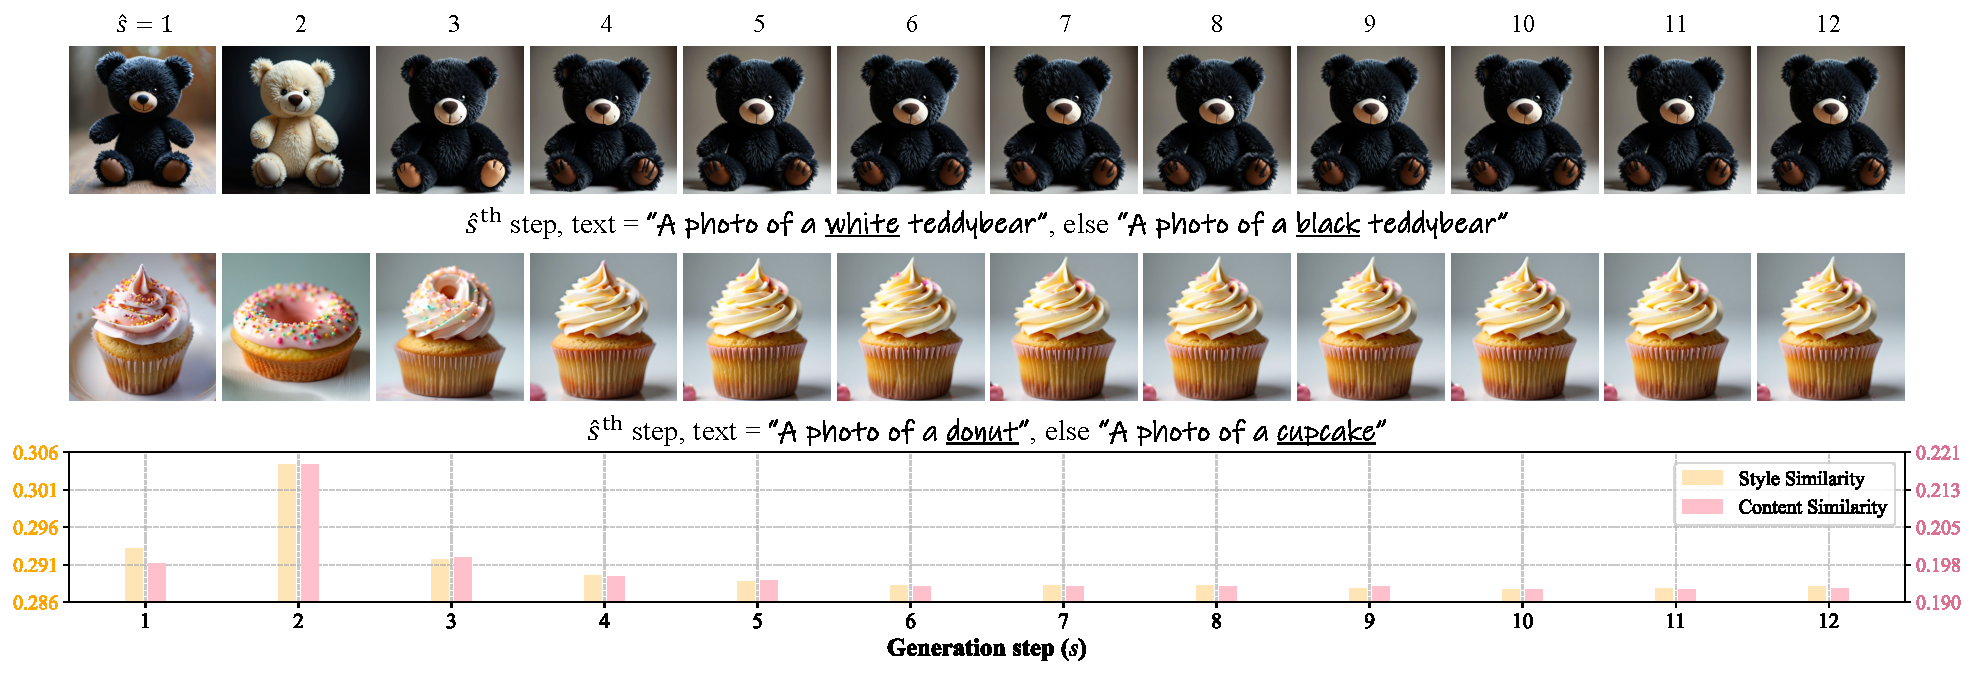
\includegraphics[width=0.7\linewidth]{Figure/observation2.pdf}
			\vspace{-0.2cm}
			\caption{Sự thay đổi độ tương đồng khi inject prompt ở các bước cụ thể.}
		\end{figure}
	\end{frame}
	
	% Slide 5: The Mathematical Breakthrough
	\begin{frame}{The Mathematical Breakthrough: SVD Trên Feature Space}
		\textbf{Tại sao lại hay?} 
		Biết được $F_3$ chứa thông tin style là chưa đủ (vì nó chứa cả content). Làm sao để tách riêng chúng ra?
		
		\begin{itemize}
			\item Phân tích suy biến (\textbf{SVD}) được áp dụng lên $F_3$: $F_3 = U \Sigma V^\top$.
			\item \textbf{Khám phá:} Nếu chỉ thay đổi \textbf{giá trị kỳ dị lớn nhất} (largest singular value $\sigma_1$), mô hình sẽ transfer \textbf{style} (màu sắc/texture) mà vẫn giữ nguyên vẹn \textbf{content} (cấu trúc đối tượng).
		\end{itemize}
	\end{frame}
	
	% Slide 6: Proposed Method - Overall Pipeline
	\begin{frame}	
		\begin{figure}
			\centering
			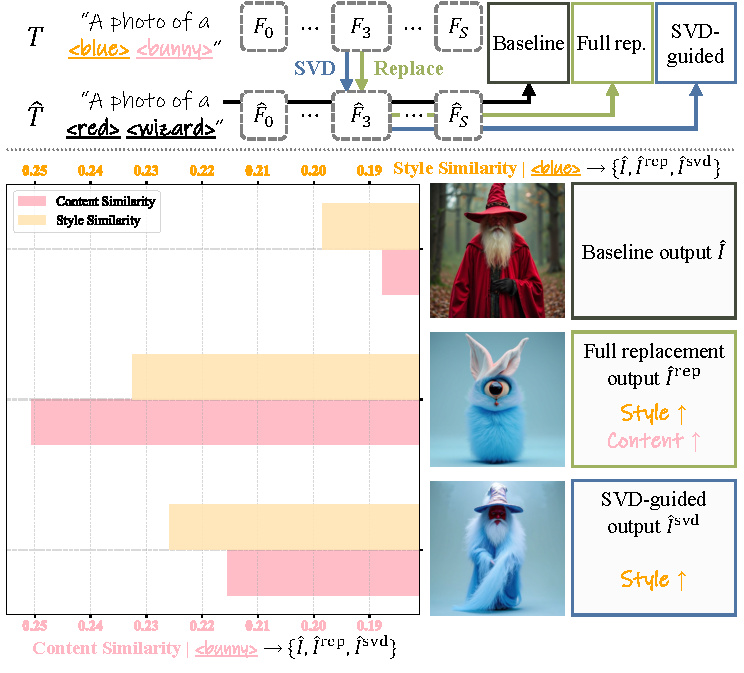
\includegraphics[width=0.6\linewidth]{Figure/observation_svd.pdf}
			\caption{SVD-guided replacement vs. Full replacement.}
		\end{figure}
	\end{frame}
	
	% Slide 6: Proposed Method - Overall Pipeline
	\begin{frame}{Method: Overall Pipeline}
		\textbf{Dual-Stream Architecture}
		\begin{itemize}
			\item Gồm \textbf{Content Path} và \textbf{Generation Path}, cả hai dùng chung một text prompt $T$ để tránh sai lệch ngữ nghĩa (semantic mismatch).
			\item Kỹ thuật điều biến (modulate) chỉ diễn ra trên \textbf{Generation Path}, sử dụng tín hiệu cấu trúc từ Content Path và style từ ảnh Reference.
		\end{itemize}
		
		\begin{figure}
			\centering
			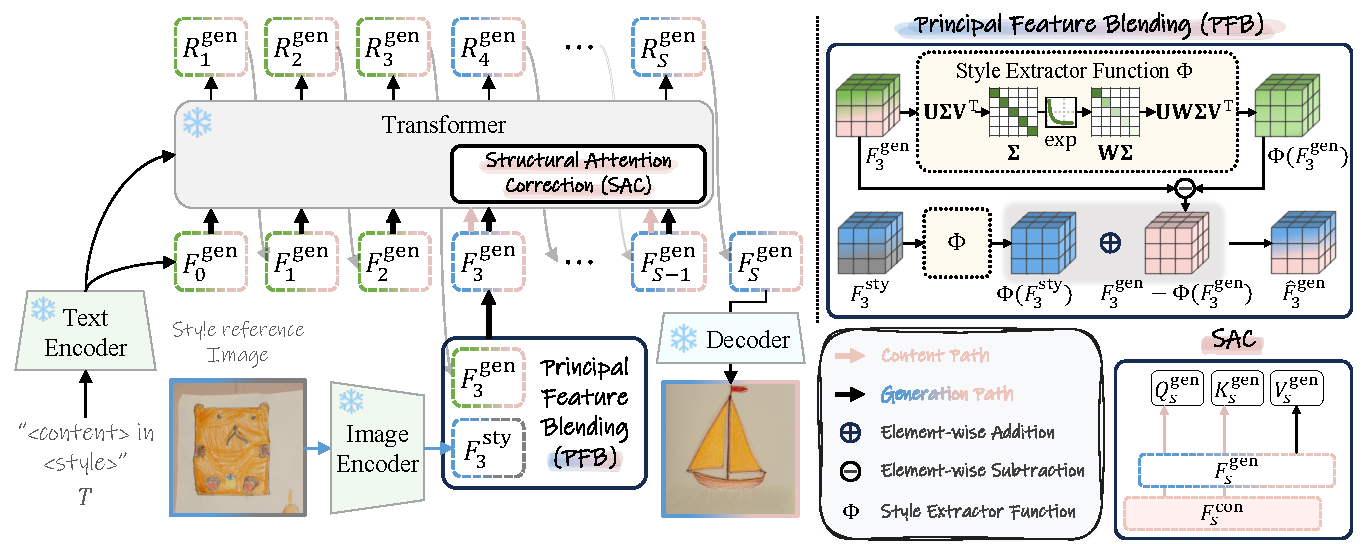
\includegraphics[width=0.85\linewidth]{Figure/pipeline_mod.pdf}
		\end{figure}
	\end{frame}
	
	% Slide 7: Module 1 - PFB
	\begin{frame}{Method: Principal Feature Blending (PFB)}
		\textbf{Mục tiêu:} Inject style một cách hiệu quả mà không làm rò rỉ nội dung (tránh content leakage) từ ảnh reference.
		\begin{itemize}
			\item Được áp dụng chính xác tại bước $s=3$ ("quân domino" số 3).
			\item Trích xuất các thành phần trọng yếu bằng hàm đánh trọng số mũ (exponential reweighting - $\Phi$):
			\begin{equation}
				\Phi(F) \triangleq \mathbf{U W \Sigma V^\top} \quad \text{với} \quad \mathbf{W} = \text{diag}(\exp^{-0 \cdot \alpha}, \dots, \exp^{-(r-1) \cdot \alpha})
			\end{equation}
			\item \textbf{Feature Update Rule (Quy tắc cập nhật):}
			\begin{equation}
				F_3^{\text{gen}} \leftarrow \Phi({F}_3^{\text{sty}}) + \big({F}_3^{\text{gen}} - \Phi({F}_3^{\text{gen}})\big)
			\end{equation}
			\item Giúp blend style chính một cách mượt mà đồng thời bảo toàn structure information gốc.
		\end{itemize}
	\end{frame}
	
	% Slide 8: Module 2 - SAC
	\begin{frame}{Method: Structural Attention Correction (SAC)}
		\textbf{Mục tiêu:} Ổn định tính mạch lạc của cấu trúc (khắc phục lỗi spatial misalignment do PFB gây ra).
		\begin{itemize}
			\item Áp dụng xuyên suốt các chặng tinh chỉnh (fine stages: $s \ge 3$).
			\item Vay mượn structural prior (\textbf{Queries} \& \textbf{Keys}) từ Content Path (luồng hoàn toàn sạch, không bị nhiễu style).
			\item \textbf{Attention Update Rule:}
			\begin{equation}
				Q_s^{\text{con}} = {W}_Q F_s^{\text{con}},\quad K_s^{\text{con}} = {W}_K F_s^{\text{con}}
			\end{equation}
			\begin{equation}
				Q_s^\text{gen} \leftarrow Q_s^\text{con}, \quad K_s^\text{gen} \leftarrow K_s^\text{con}
			\end{equation}
			\item \textit{Kết quả:} \textbf{Generation Path} tập trung sự \textbf{attention} vào đúng các vùng không gian trong khi render style mới.
		\end{itemize}
	\end{frame}
	
	% Slide 9: Experimental Setup
	\begin{frame}{Experimental Setup \& Metrics}
		\begin{itemize}
			\item \textbf{Dataset:} 190 prompts từ Parti + 10 representative styles (theo giao thức của FineStyle).
			\item \textbf{Baselines:} 
			\begin{itemize}
				\item Dựa trên Tuning: StyleDrop, DreamStyler, DB-LoRA, B-LoRA
				\item Training-free: IP-Adapter, StyleAligned, CSGO, StyleAR
			\end{itemize}
			\item \textbf{Metrics:}
			\begin{itemize}
				\item $S_{\text{txt}}$: CLIP Text score (Đo lường Prompt Fidelity).
				\item $S_{\text{img}}$: CLIP Image score (Đo lường Style Fidelity).
				\item $S_{\text{harmonic}}$: Trung bình điều hòa của $S_{\text{txt}}$ và $S_{\text{img}}$ (Đánh giá độ cân bằng).
			\end{itemize}
		\end{itemize}
	\end{frame}
	
	% Slide 10: Quantitative Results
	\begin{frame}{Quantitative Results}
		\begin{itemize}
			\item \textbf{Tốc độ:} Nhanh hơn 195$\times$ so với các phương pháp tuning (3.58s so với 698s).
			\item \textbf{Sự cân bằng:} Đạt Harmonic Score cao nhất ($0.437$), duy trì prompt fidelity xuất sắc mà không bị dính lỗi \textbf{content leakage}.
		\end{itemize}
		\vspace{0.3cm}
		\begin{table}
			\centering
			\resizebox{\textwidth}{!}{
				\begin{tabular}{c|c|cccccccc}
					\toprule
					Metric & \textbf{Ours} & IP-Adapter & StyleAligned & DreamStyler & DB-LoRA & B-LoRA & CSGO & StyleAR \\
					\midrule
					Training-Free & \textbf{Yes} & Yes & Yes & No & No & No & Yes & Yes \\ 
					$S_{\text{harmonic}} \uparrow$ & \textbf{0.437} & 0.433 & 0.438 & 0.403 & 0.420 & 0.410 & 0.421 & 0.434 \\
					$S_{\text{txt}} \uparrow$ & \textbf{0.334} & 0.302 & 0.315 & 0.304 & 0.323 & 0.324 & 0.318 & 0.314 \\
					$S_{\text{img}} \uparrow$ & 0.630 & 0.763 & 0.716 & 0.599 & 0.602 & 0.559 & 0.623 & 0.701 \\
					Thời gian (s) $\downarrow$ & \textbf{3.58} & 10.13 & 64.58 & 698.98 & 342.01 & 630.42 & 15.87 & 346.68 \\
					\bottomrule
			\end{tabular}}
		\end{table}
	\end{frame}
	
	% Slide 11: Qualitative Results
	\begin{frame}{Qualitative Results}
		\begin{figure}
			\centering
			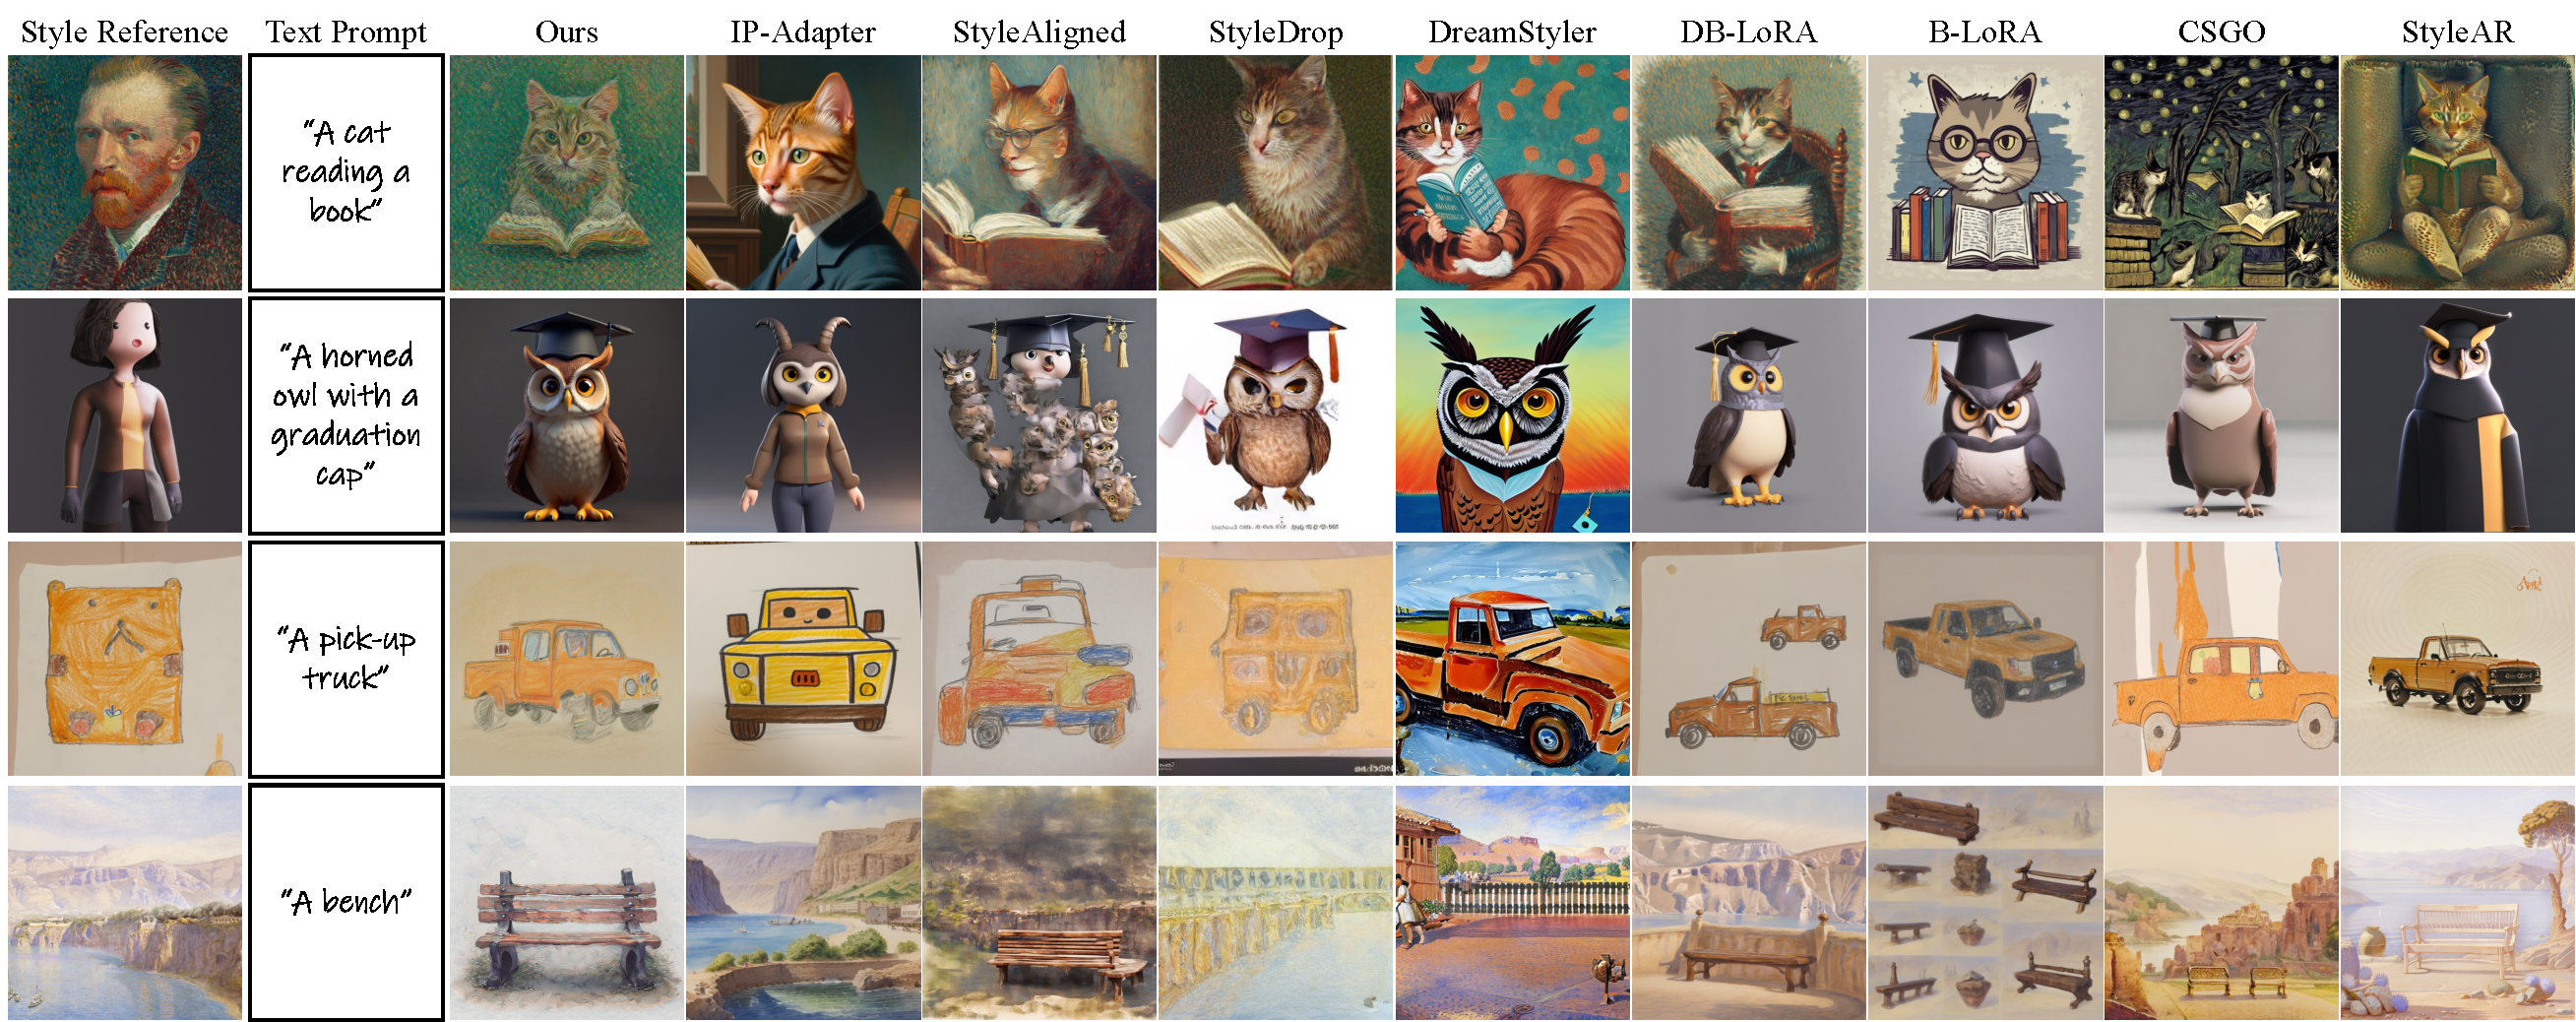
\includegraphics[height=0.7\textheight]{Figure/qual_results2.pdf}
		\end{figure}
	\end{frame}
	
	% Slide 12: Ablation Study
	\begin{frame}{Ablation Study: PFB \& SAC}
		\begin{itemize}
			\item \textbf{(b) Full Replacement:} Điểm style cực cao nhưng phá hủy hoàn toàn prompt fidelity (bị content leakage).
			\item \textbf{(c) Chỉ sử dụng PFB:} Điểm cân bằng tốt hơn nhờ trích xuất style qua \textbf{SVD} thay vì lấy toàn bộ feature.
			\item \textbf{(d) PFB + SAC (Ours):} Cơ chế \textbf{Attention Correction} giúp khôi phục semantic alignment và giữ đúng hình dáng vật thể.
		\end{itemize}
		\begin{figure}
			\centering
			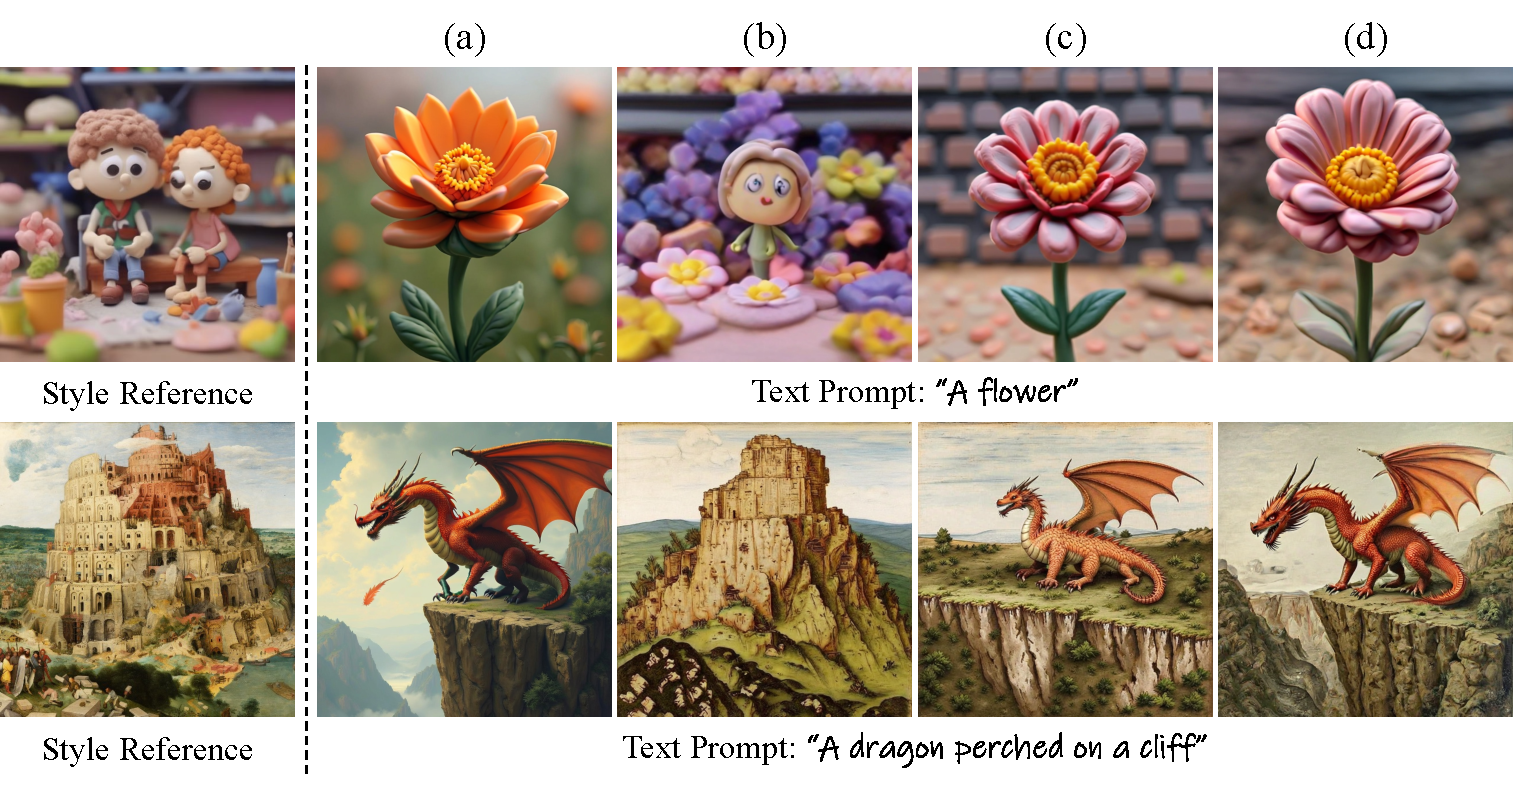
\includegraphics[width=0.6\linewidth]{Figure/ablation.pdf}
		\end{figure}
	\end{frame}
	
	% Slide 13: Critical Review
	\begin{frame}{Strength \& Weakness}
		\textbf{Điểm Mạnh:}
		\begin{itemize}
			\item \textbf{Cực kỳ nhanh:} Framework \textbf{training-free} + kết hợp \textbf{autoregressive model} giúp loại bỏ hoàn toàn độ trễ của diffusion steps.
			\item \textbf{Phương pháp Interpretable:} Tiếp cận dựa trên phân tích toán học (\textbf{SVD}) trong \textbf{feature space}, không phải kiểu "black-box" prompt tuning.
			\item \textbf{Disentanglement tốt:} Xử lý triệt để bài toán content leakage nhờ khả năng tách bạch style/content bằng cơ chế attention luồng kép.
		\end{itemize}
		\vspace{0.3cm}
		\textbf{Điểm Yếu:}
		\begin{itemize}
			\item \textbf{Style không đồng nhất:} Mô hình gặp khó khi ảnh reference chứa nhiều style xung đột (do thuật toán \textbf{SVD} sẽ có xu hướng hòa trộn tất cả thành một dominant component duy nhất).
		\end{itemize}
	\end{frame}
	
	% Slide 14: Conclusion
	\begin{frame}{Conclusion \& Contributions}
		\begin{itemize}
			\item Phân tích và chứng minh được \textbf{feature ở Bước 3} trong \textbf{autoregressive models} là điểm chốt chặn cho cả nội dung và phong cách.
			\item Phát hiện ra rằng \textbf{dominant singular values (SVD)} của feature này có thể cô lập style một cách hoàn hảo.
			\item Đề xuất 2 module \textbf{PFB} và \textbf{SAC} để inject style và ổn định structure mà không tốn chi phí training.
			\item Đạt chất lượng visual ngang ngửa với các mô hình SOTA fine-tuning nhưng thời gian inference thực tế chỉ mất 3.58 giây.
		\end{itemize}
	\end{frame}
	
\end{document}